%%%%%%%%%%%%%%%%%%%%%%%%%%%%%%%%%%%%%%%%%%%%%%%%%%%%%%%%%%%%%%%%%%%%%%%%%%%%%%%%
%%  Rapport de Service, WorkflowManagement
%%%%%%%%%%%%%%%%%%%%%%%%%%%%%%%%%%%%%%%%%%%%%%%%%%%%%%%%%%%%%%%%%%%%%%%%%%%%%%%%
\documentclass[11pt, a4paper]{article}

\usepackage[english]{babel}
\usepackage[utf8]{inputenc}
\usepackage[T1]{fontenc}
\usepackage{amsfonts}
\usepackage{fancyhdr}
\usepackage[margin={2.5cm, 2.5cm}]{geometry}
\usepackage{graphicx}
\usepackage{pdfpages}
\usepackage{hyperref}
% \usepackage{algorithm2e}

\hypersetup{
  colorlinks,
  citecolor=black,
  filecolor=black,
  linkcolor=black,
  urlcolor=black
}

\newcommand\note[1]{\begin{quote}\emph{\textbf{Note : }}#1\end{quote}}

\pagestyle{empty}
\fancyhf{}
\renewcommand{\headrulewidth}{0pt}
\renewcommand{\footrulewidth}{0pt}
\lhead{Logoot : a Scalable Optimistic Replication Algorithm for Collaborative Editing}
\rhead{}
\lfoot{\today}
\cfoot{\thepage}
\rfoot{}

%%%%%%%%%%%%%%%%%%%%%%%%%%%%%%%%%%%%%%%%%%%%%%%%%%%%%%%%%%%%%%%%%%%%%%%%%%%%%%%%
%% Préambule
%%%%%%%%%%%%%%%%%%%%%%%%%%%%%%%%%%%%%%%%%%%%%%%%%%%%%%%%%%%%%%%%%%%%%%%%%%%%%%%%
\title{ Summary
       <<Logoot : a Scalable Optimistic Replication Algorithm for Collaborative Editing on P2P Networks>>}

\author{Adrien Drouet\\Alexandre Prenza}
\date{Year 2011-2012\\
      (University of Nantes)}
\makeindex

%%%%%%%%%%%%%%%%%%%%%%%%%%%%%%%%%%%%%%%%%%%%%%%%%%%%%%%%%%%%%%%%%%%%%%%%%%%%%%%%
%% Début
%%%%%%%%%%%%%%%%%%%%%%%%%%%%%%%%%%%%%%%%%%%%%%%%%%%%%%%%%%%%%%%%%%%%%%%%%%%%%%%%
\begin{document}
  \maketitle

  \fancypagestyle{plain}{\fancyhead{} \fancyfoot{}} 
  %\vfill
  %\tableofcontents\renewcommand{\headrulewidth}{0.4pt}
  ~\newline
  \renewcommand{\footrulewidth}{0.4pt}
  \pagestyle{fancy}
  \fancypagestyle{plain}{}
  \newpage

%%%%%%%%%%%%%%%%%%%%%%%%%%%%%%%%%%%%%%%%%%%%%%%%%%%%%%%%%%%%%%%%%%%%%%%%%%%%%%
 Nowodays, massive collaborative editing becomes a reality through leading projects such as Wikipedia. By this way, real-time editing systems are catching on, enabling multiple authors to edit the same document at the same time, whenever they are and whenever it is.
 
 Any real-time editing have to ensure the CCI\footnote{Causality, Convergence, and Intention preservation}, and should scale according to the number of users and to the nuber of edits. Actually, existing approaches to build distributed collaborative editing systems either do not scale in one of these.  
 
 \emph{WOOKI} and \emph{TreeDoc} are two collaborative editing system known which ensure the CCI but also to scale according to the number of users in the network. Both are different, but both kept deleted lines using tombstones. 
 
 According to the scalability definition, the tombstone cost is not acceptable on massive editing systems. For instance, for the most edited pages of Wikipedia, the tombstone storage overhead can represent several hundred of times the document size. Tombstones are also responsible of performance degradation.
 
 The purpose of this paper is to explain a new approach to build distributed colaborative editing systems, \emph{Logoot}, which scales in terms of number of users, but also in terms of number of edits, removing the principle of tombstones. \emph{Logoot} also ensure the CCI criteria.
 
 After some explanations about how \emph{Logoot} is working and how it scales and ensures the CCI as a P2P collaborative editing system, it will be evaluated and compared with some others collaborative editing systems like \emph{WOOKI} and \emph{TreeDoc} on a set of the most edited and the biggest pages of Wikipedia.

 A collaborative editing system is considered correct if it respects the CCI criteria:
 \begin{itemize}
  \item Causality: It ensures that all operations ordrered by a precedence relation will be executed in the same order on every copy.
  \item Convergence/Consistency : It ensure that the system converges ; all replicas are identical.
  \item Intention : The expected effect must be observed on all replicas.
  \item Scalability : The system must handle the addition of users or objects without suffering a noticeable loss of performance.
 \end{itemize}

 \emph{WOOKI} is a P2P wiki system, based on \emph{Wooto} representing documents like a Hasse diagram. It barely respects the CCI correction criteria, replacing Causality by preconditions. Convergence will be ensured by using tombstones when a line is deleted.

 \emph{TreeDoc} is another collaborative editing system using a binary tree to represent the document. Here, again, deleted lines are also kept using tombstones. A procedure is proposed to remove tombstones, but it cannot be used in open-network such as P2P environments.

 The main idea of \emph{Logoot} is to use a data type where all concurrent operations commute. Combined with the respect of the causality between operations, this commutation ensures the convergence criteria. To ensure commutativity on a linear structure, the solution is based on a total order between every elements. There is two kinds of modification :
 \begin{itemize}
  \item \emph{insert(pid, text)} that inserts the line content \emph{text} at the position identifier \emph{pid}.
  \item \emph{delete(pid)} that removes the line at the position identifier \emph{pid}. 
 \end{itemize}

 A \emph{Logoot} document is composed by \emph{lines} defined by an \emph{identifier} and a \emph{content}. The content is simply a text line while the identifier is a unique \emph{position identifier}. It must be unique to ensure operations to commute. Since a user can always insert a line, the model need to be able to generate a position A such as P < A < N for any P and N.

 Every line is represented by a list of \emph{identifiers} and a clock incremented on each site each time a line is created. An \emph{identifier} is a list of couple \emph{(position, site)} where \emph{position} is an integer and \emph{site} a site identifier.

 This exemple show the insertion of three lines from differents site. First, the site (1) insert a line, generating \emph{<1,1>,0}, reprensenting the position 1, the site 1, and the clock 0. Then another site insert a line, generating \emph{<1,3>,2}. Finally, a last site try to insert another line between these two. Looking that it is imposible to find any integer between 1 and 1, another \emph{position, site} is added to the list, generating \emph{<1,1>.<1,5>,3} where \emph{<1,1>} is the previous position, and \emph{<1,5>,3} another position added. 
 \begin{verbatim}
  0. <0,0> - The begining of the document
  1. <1,1>,0, "First line insered on a site (1)"
  3. <1,1>.<1,5>,3 "A last line insered between two line by another site (5)" 
  2. <1,3>,2, "Another line insered from a different site (3)"
  0. <MAXINT,0> - The end of the document
 \end{verbatim}
 
 Looking that every line have a different unique identifier, tombstone are not anymore needed to ensure the convergence of the document.

 The size of a \emph{Logoot position identifier} is unbounded, because theoretically, it can grow each time a line is inserted. On the worst case, the size of the document model overhead can be \emph{O(n\textsuperscript{2})} where n is the total number of inserted lines, but the probability of this case is negligible.

 And finally, applying \emph{Logoot}, \emph{Wooto} and \emph{TreeDoc} on the most edited pages and the biggest pages of Wikipedia shows that the \emph{Logoot} overhead is inferior to the document while tombstones based approaches are more than 100 times the document size and continuously grows.

 \begin{figure}[h!]
  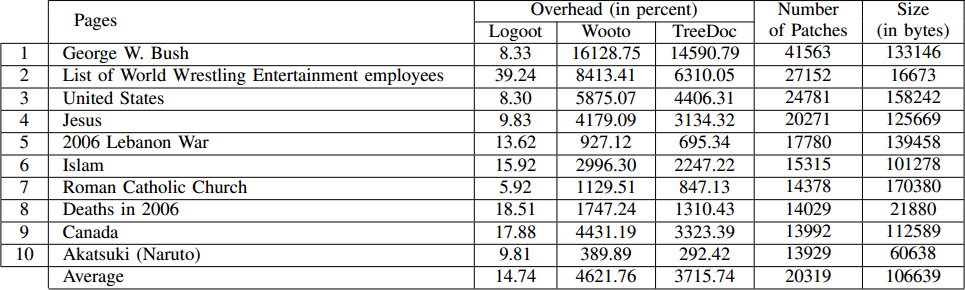
\includegraphics[width=1\textwidth]{includes/etu1}
  \caption{Most edited encyclopedic pages}
  \label{fig:etu1}
 \end{figure}

 \begin{figure}[h!]
  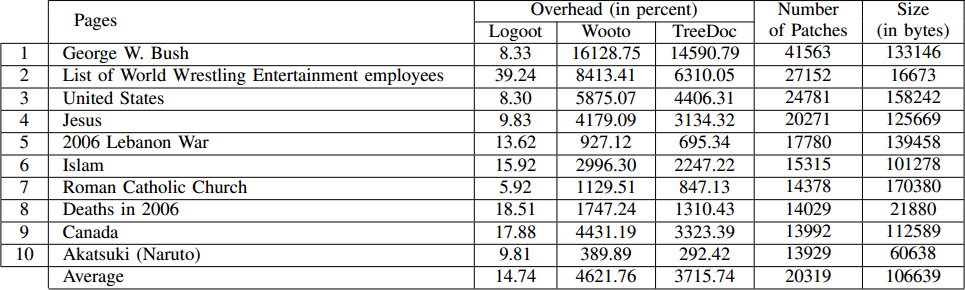
\includegraphics[width=1\textwidth]{includes/etu1}
  \caption{Most edited pages}
  \label{fig:etu2}
 \end{figure}

 \begin{figure}[h!]
  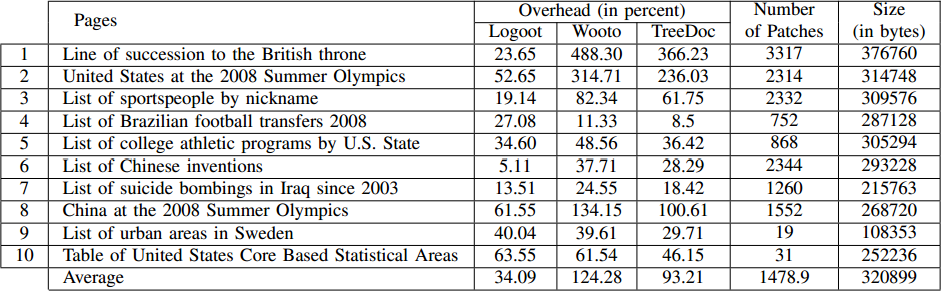
\includegraphics[width=1\textwidth]{includes/etu3}
  \caption{Biggest pages}
  \label{fig:etu3}
 \end{figure}

 We can see on the figures \ref{fig:etu1} and \ref{fig:etu2} that most edited encyclopedic pages, and even more, on most edited pages that \emph{Logoot} is far better than \emph{Wooto} and \emph{TreeDoc}, looking that both of them have to keep thousands of tombstones while \emph{Logoot} does not keep anything for any removed line.

 However, on the figure \ref{fig:etu3} representing the biggest pages, the power of \emph{Logoot} is less noticeable because there is not many removed line, but it is still better than \emph{Wooto} and \emph{TreeDoc} on the average.

 To conclude, \emph{Logoot} is an optimistic replication algorithm that ensure the CCI consistency, and can be used on structured or unstructured P2P networks. It does not require tombstones and the experimentations have shown that \emph{Logoot} has better average performances than the \emph{WOOT} and the \emph{TreeDoc} algorithms.
%%%%%%%%%%%%%%%%%%%%%%%%%%%%%%%%%%%%%%%%%%%%%%%%%%%%%%%%%%%%%%%%%%%%%%%%%%%%%%
\end{document}

